% Share |N_k| / |N_n| of the Dynasearch moves contained in N_k (exact, from the recurrence).
% Dashed markers: k = floor(log2 n) + 2.
\documentclass[border=2pt]{standalone}
\usepackage{pgfplots}
\pgfplotsset{compat=1.18}
\begin{document}
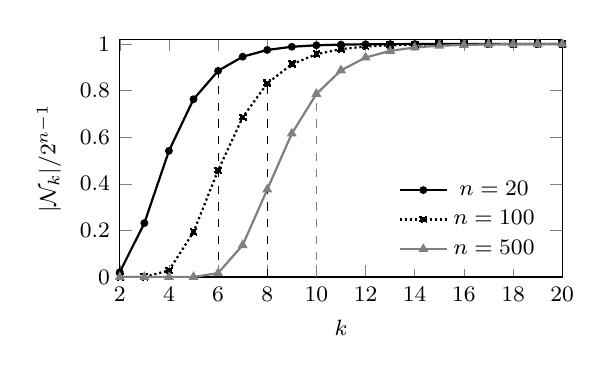
\begin{tikzpicture}
\begin{axis}[width=7.2cm,height=4.6cm,xmin=2,xmax=20,ymin=0,ymax=1.02,
  xlabel={$k$},ylabel={$|\mathcal N_k|/2^{n-1}$},xtick={2,4,...,20},
  legend pos=south east,legend style={font=\footnotesize,draw=none},
  tick label style={font=\footnotesize},label style={font=\footnotesize}]
\addplot[thick,mark=*,mark size=1pt] coordinates {(2,0.0209)(3,0.2316)(4,0.5416)(5,0.7631)(6,0.8849)(7,0.9456)(8,0.9746)(9,0.9883)(10,0.9946)(11,0.9976)(12,0.9989)(13,0.9995)(14,0.9998)(15,0.9999)(16,1)(17,1)(18,1)(19,1)(20,1)};
\addplot[thick,densely dotted,mark=square*,mark size=1pt] coordinates {(2,0)(3,0.0003)(4,0.0283)(5,0.1932)(6,0.4577)(7,0.6852)(8,0.8314)(9,0.9133)(10,0.9563)(11,0.9782)(12,0.9892)(13,0.9946)(14,0.9973)(15,0.9987)(16,0.9994)(17,0.9997)(18,0.9998)(19,0.9999)(20,1)};
\addplot[thick,gray,mark=triangle*,mark size=1.3pt] coordinates {(2,0)(3,0)(4,0)(5,0.0002)(6,0.0169)(7,0.1369)(8,0.3756)(9,0.6157)(10,0.7859)(11,0.887)(12,0.942)(13,0.9706)(14,0.9852)(15,0.9926)(16,0.9963)(17,0.9982)(18,0.9991)(19,0.9995)(20,0.9998)};
\legend{$n=20$,$n=100$,$n=500$}
\draw[dashed,thin] (axis cs:6,0) -- (axis cs:6,0.8849);
\draw[dashed,thin] (axis cs:8,0) -- (axis cs:8,0.8314);
\draw[dashed,thin,gray] (axis cs:10,0) -- (axis cs:10,0.7859);
\end{axis}
\end{tikzpicture}
\end{document}
